\chapter{User Interface Design}
\label{cha:ui}
In this section, we show an overall view of the different user interfaces of Travlendar+ for each client. The UX diagram shows both the user flow and the different screens of the application (illustrated in Figure \ref{fig:generaluxdiag}). 
In Figure \ref{fig:mobileuxdiag} the User Interface of the mobile implementation integrating the user flow across Travlendar+ is shown. In Figures \ref{fig:landingmockupweb}, \ref{fig:loginmockupweb} and \ref{fig:maindashmockupweb} we show some mockups related to the web application. As can be seen, user interface of the web and mobile application are meant to be as similar as possible so that a continuous experience across the clients can be provided.

The general UX Diagram is composed of 2 parts:
\begin{itemize}
\item The \textbf{white} one describes the common functionalities of the web and mobile implementation.
\item The \textbf{yellow} one describes the functionalities implemented only by the mobile client.
\end{itemize}


\begin{figure}
	\centering
	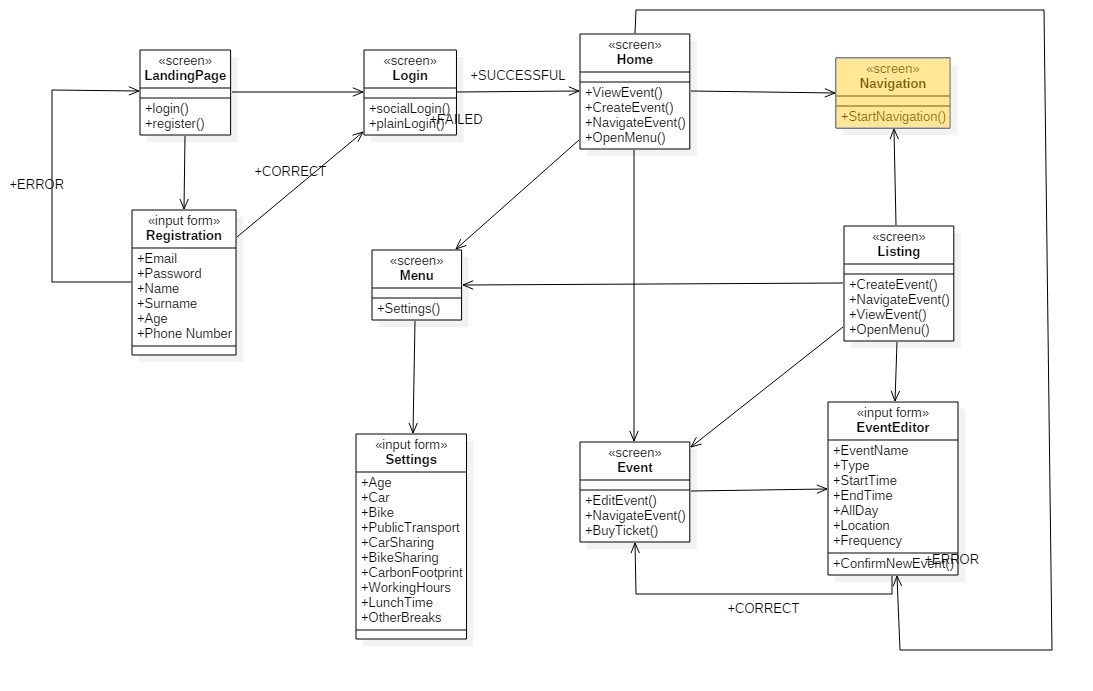
\includegraphics[width=6in]{./diagrams/GeneralUxDiagram.jpg}
	\caption{UX Diagram of the client implementation.}
	\label{fig:generaluxdiag}
\end{figure}
\begin{figure}
	\centering
	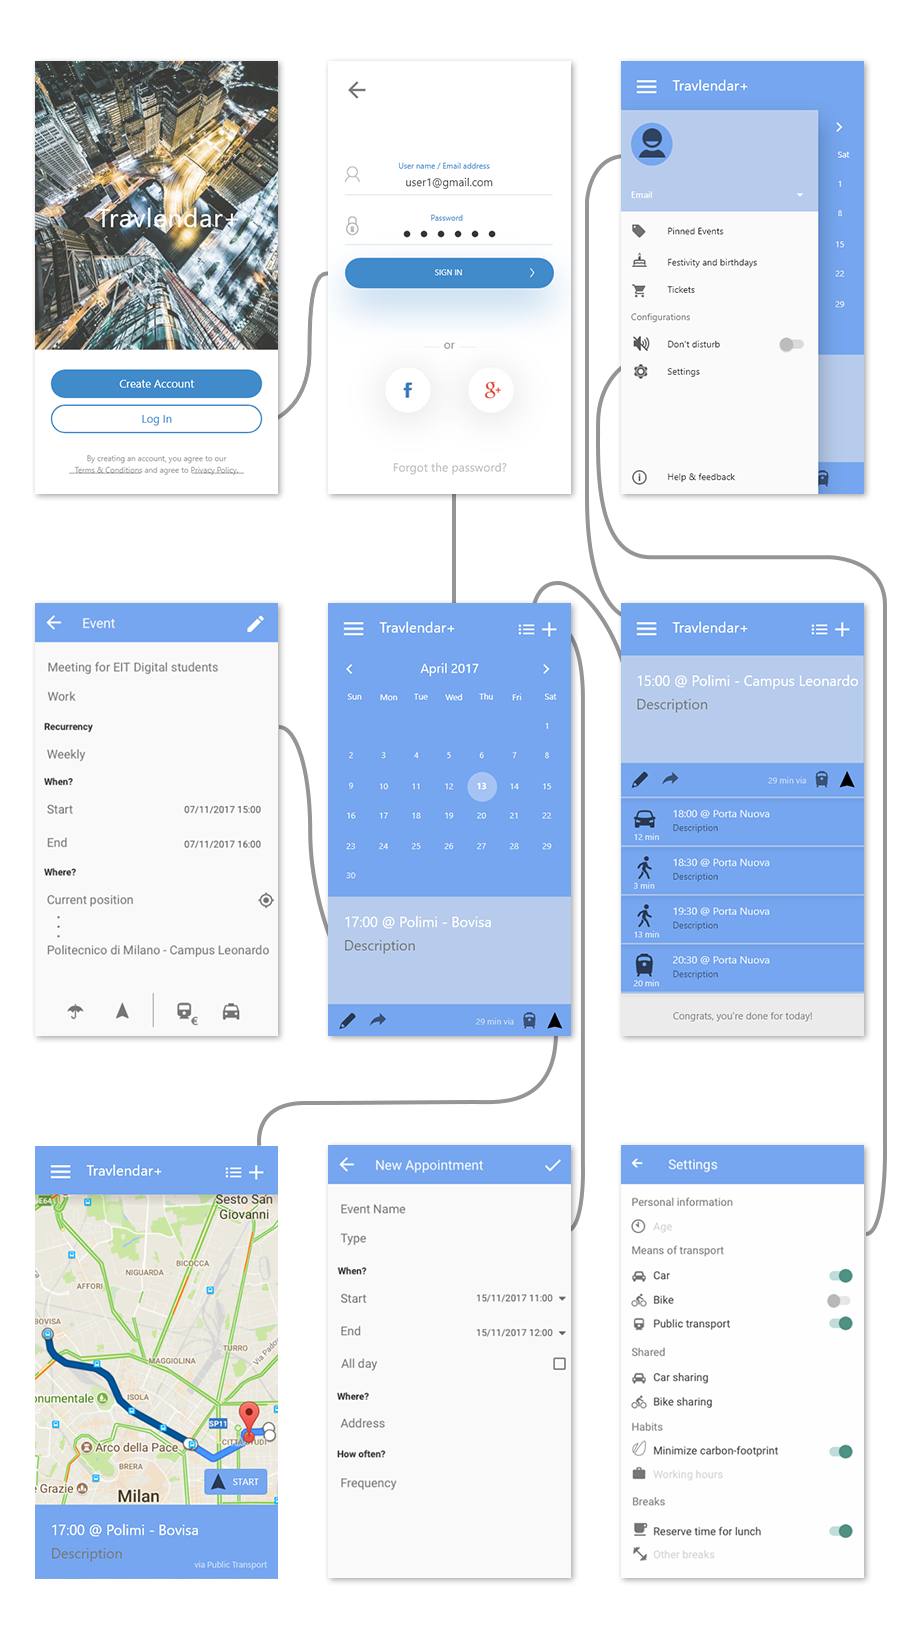
\includegraphics[width=5.4in]{./diagrams/MobileUxDiagram.png}
	\caption{UI	Diagram for the mobile implementation.}
	\label{fig:mobileuxdiag}
\end{figure}

\begin{figure}
	\centering
	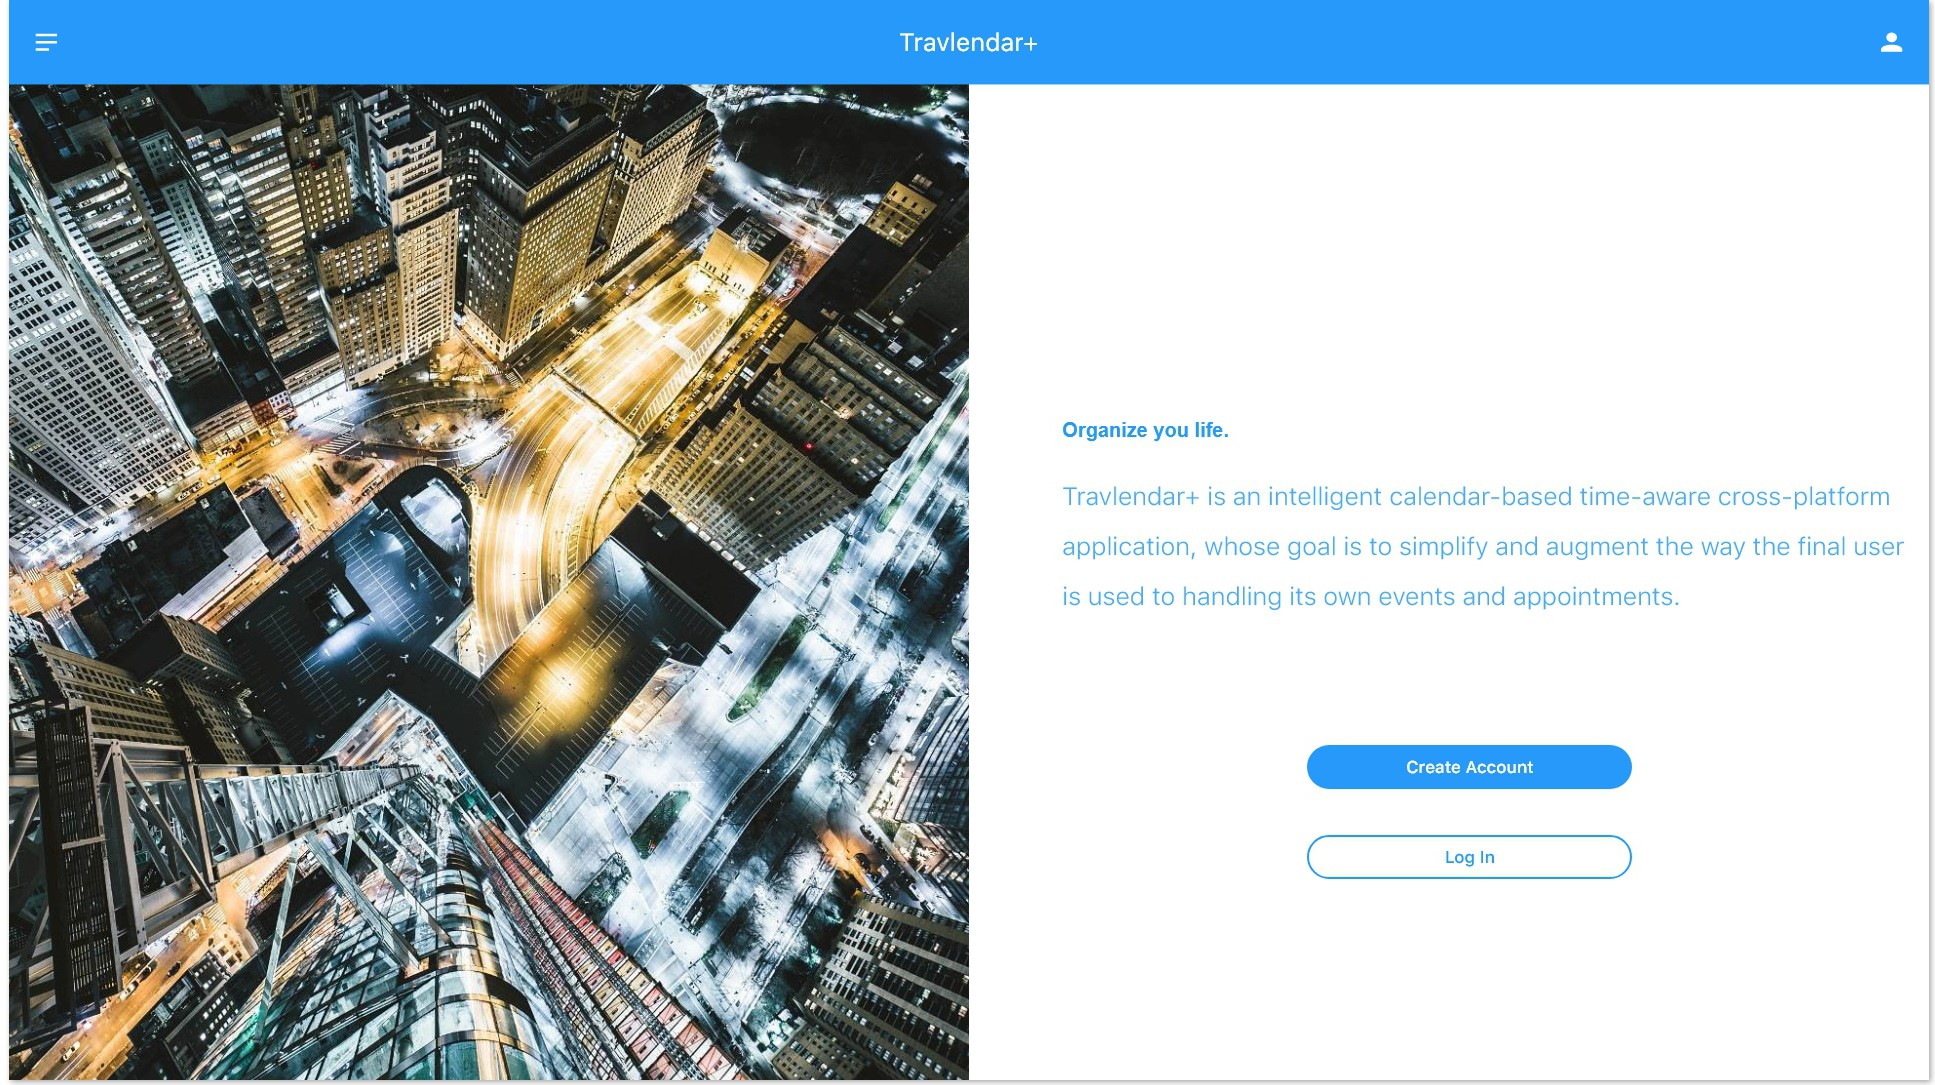
\includegraphics[width=7.5in]{./diagrams/LandingMockupWeb.jpg}
	\caption{Mockup of the landing page for the web application.}
	\label{fig:landingmockupweb}
\end{figure}

\begin{figure}
	\centering
	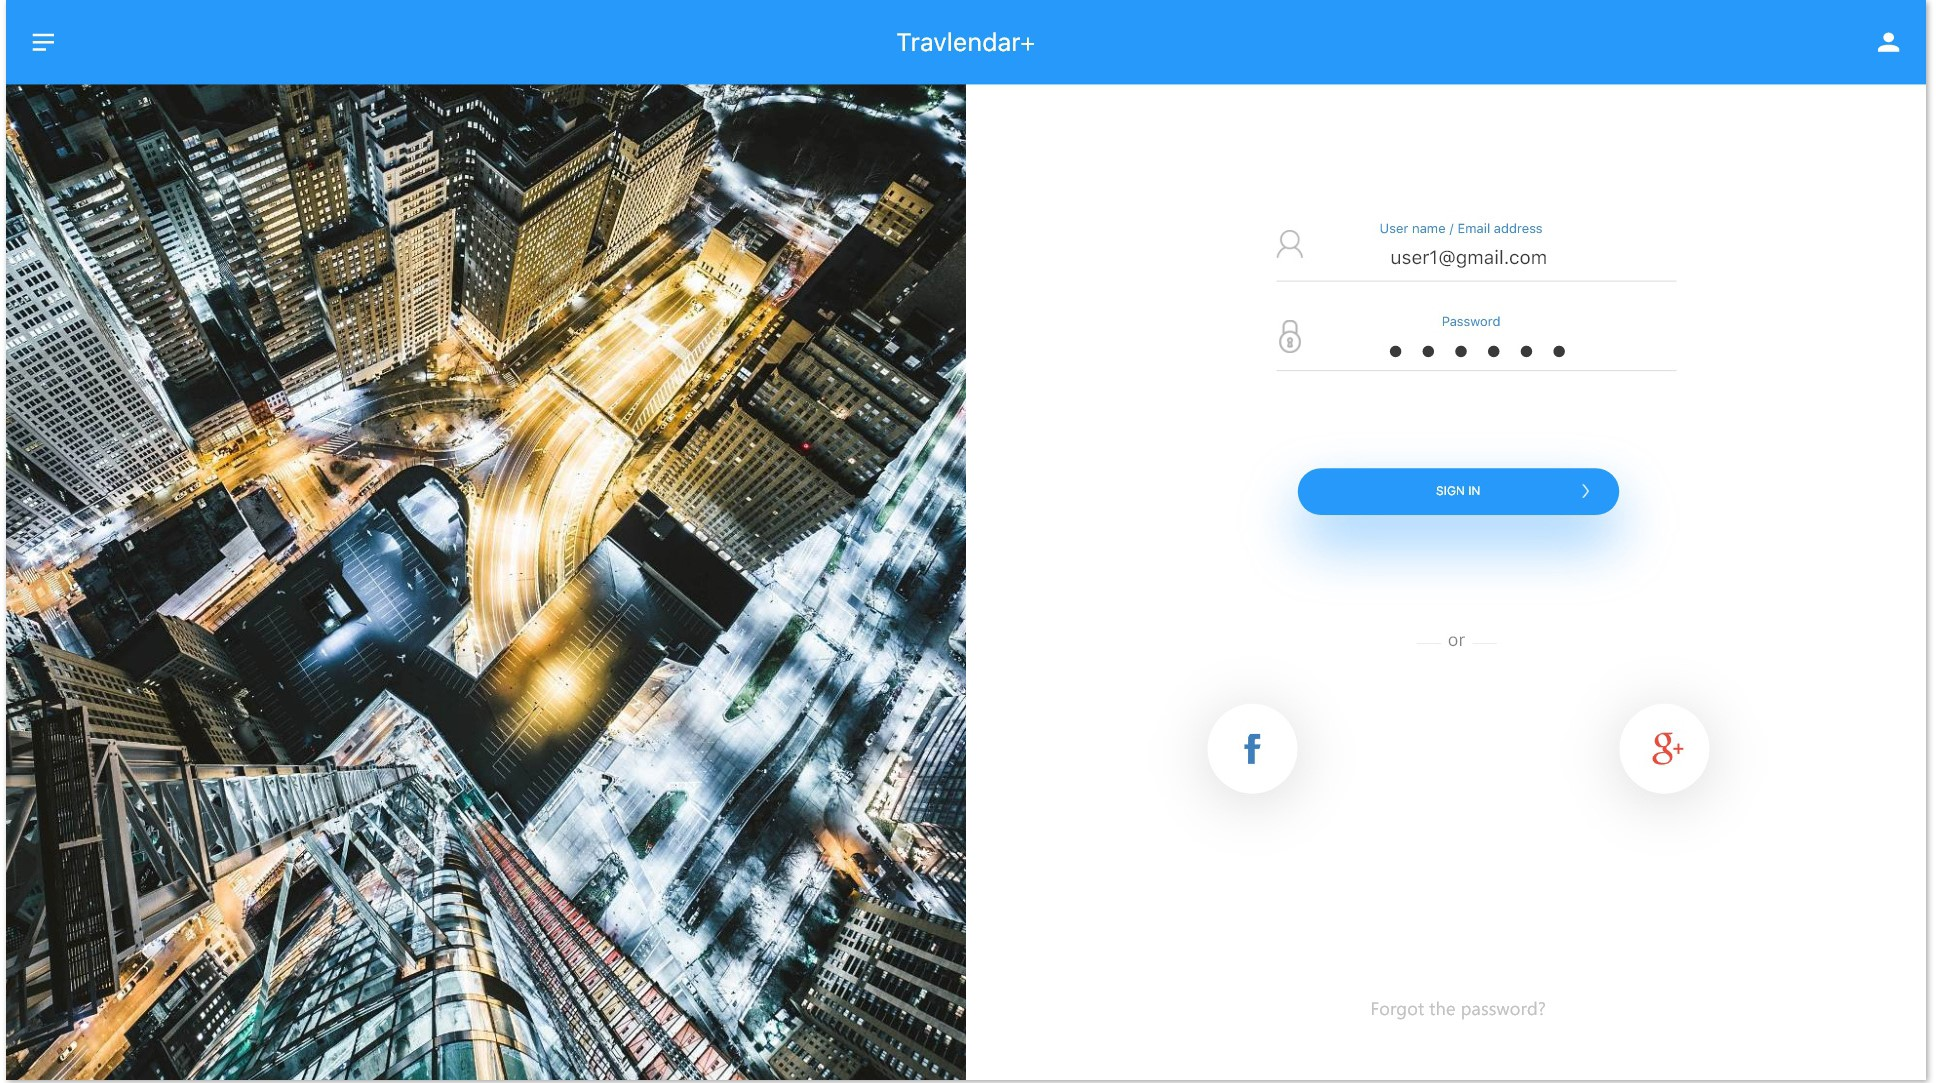
\includegraphics[width=7.5in]{./diagrams/LoginMockupWeb.jpg}
	\caption{Mockup of the login page for the web application.}
	\label{fig:loginmockupweb}
\end{figure}

\begin{figure}
	\centering
	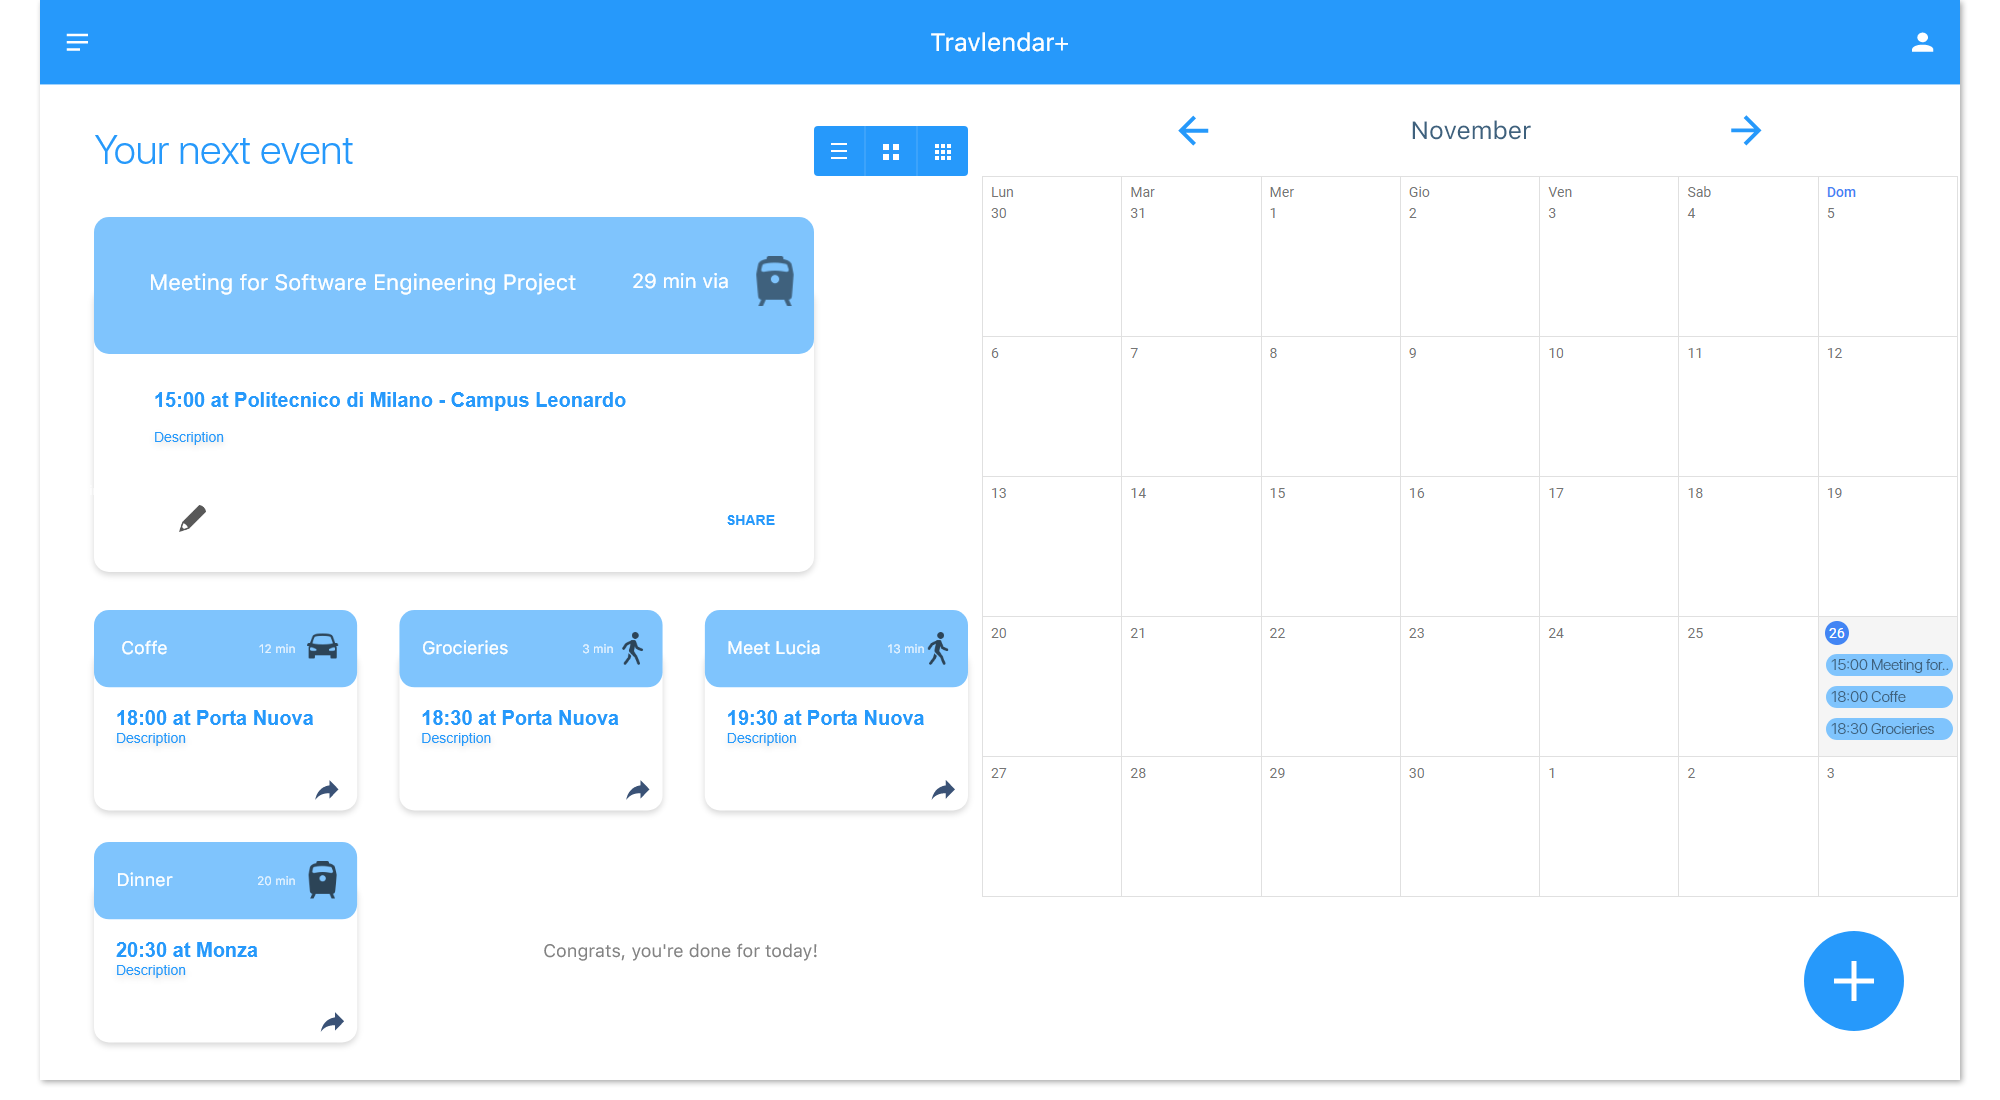
\includegraphics[width=7.5in]{./diagrams/MainDashMockupWeb.png}
	\caption{Mockup of the main dash page for the web application.}
	\label{fig:maindashmockupweb}
\end{figure}